Una vez se ha realizado la instalación de la aplicación por medio del fichero APK, será posible comenzar a utilizarla. Al lanzarla por primera vez, en función de la versión del sistema operativo Android, se lanzarán alertas para conceder permisos de cara al envío de notificaciones, la ubicación y la gestión de archivos de imagen. Es recomendable habilitar todos ellos mientras la app esté en uso para evitar problemas de funcionamiento y aprovechar todas las características.

\subsection{Inicio de sesión y registro de usuarios}

Tras aceptar los permisos, se mostrará la pantalla de inicio de sesión representada en la Figura \ref{fig:login}. Es posible hacer uso de la cuenta de demostración, usando “\texttt{demo}” como usuario y contraseña, si bien también puede pulsarse sobre el enlace de registro para dar de alta un nuevo usuario, como representa la Figura \ref{fig:signup}. En caso de elegir esta opción, deberá indicarse un nombre de usuario que no puede existir ya en la base de datos de la aplicación, así como una contraseña con 4 o más caracteres que, por motivos de seguridad, deberá introducirse dos veces.

Tras haber creado una nueva cuenta de usuario, se redirigirá a la pantalla de inicio de sesión, donde será posible iniciar sesión usando el usuario y la contraseña registradas. Basta con completar los campos y pulsar sobre el botón “Iniciar sesión” para acceder a la aplicación.

La pantalla de bienvenida de la Figura \ref{fig:fichado} ilustra una situación de fichaje en curso. La navegación por medio de los distintos apartados de la aplicación se realiza presionando sobre el botón de las tres líneas que se muestra en la esquina superior izquierda. La aplicación presenta tres áreas separadas sobre las que se darán más detalles a continuación:

\begin{itemize}
    \item \textbf{Fichar}: permite consultar el estado de un fichaje en curso o fichar a medida.
    \item \textbf{Historial}: ofrece información sobre los fichajes almacenados, además de permitir exportar e importar datos.
    \item \textbf{Ajustes}: permite definir aspectos de configuración a nivel de la aplicación. Para obtener la mejor experiencia de usuario, se recomienda comenzar accediendo a esta sección.
\end{itemize}

\begin{figure}[H]
     \centering
     \begin{subfigure}[b]{0.3\textwidth}
         \centering
         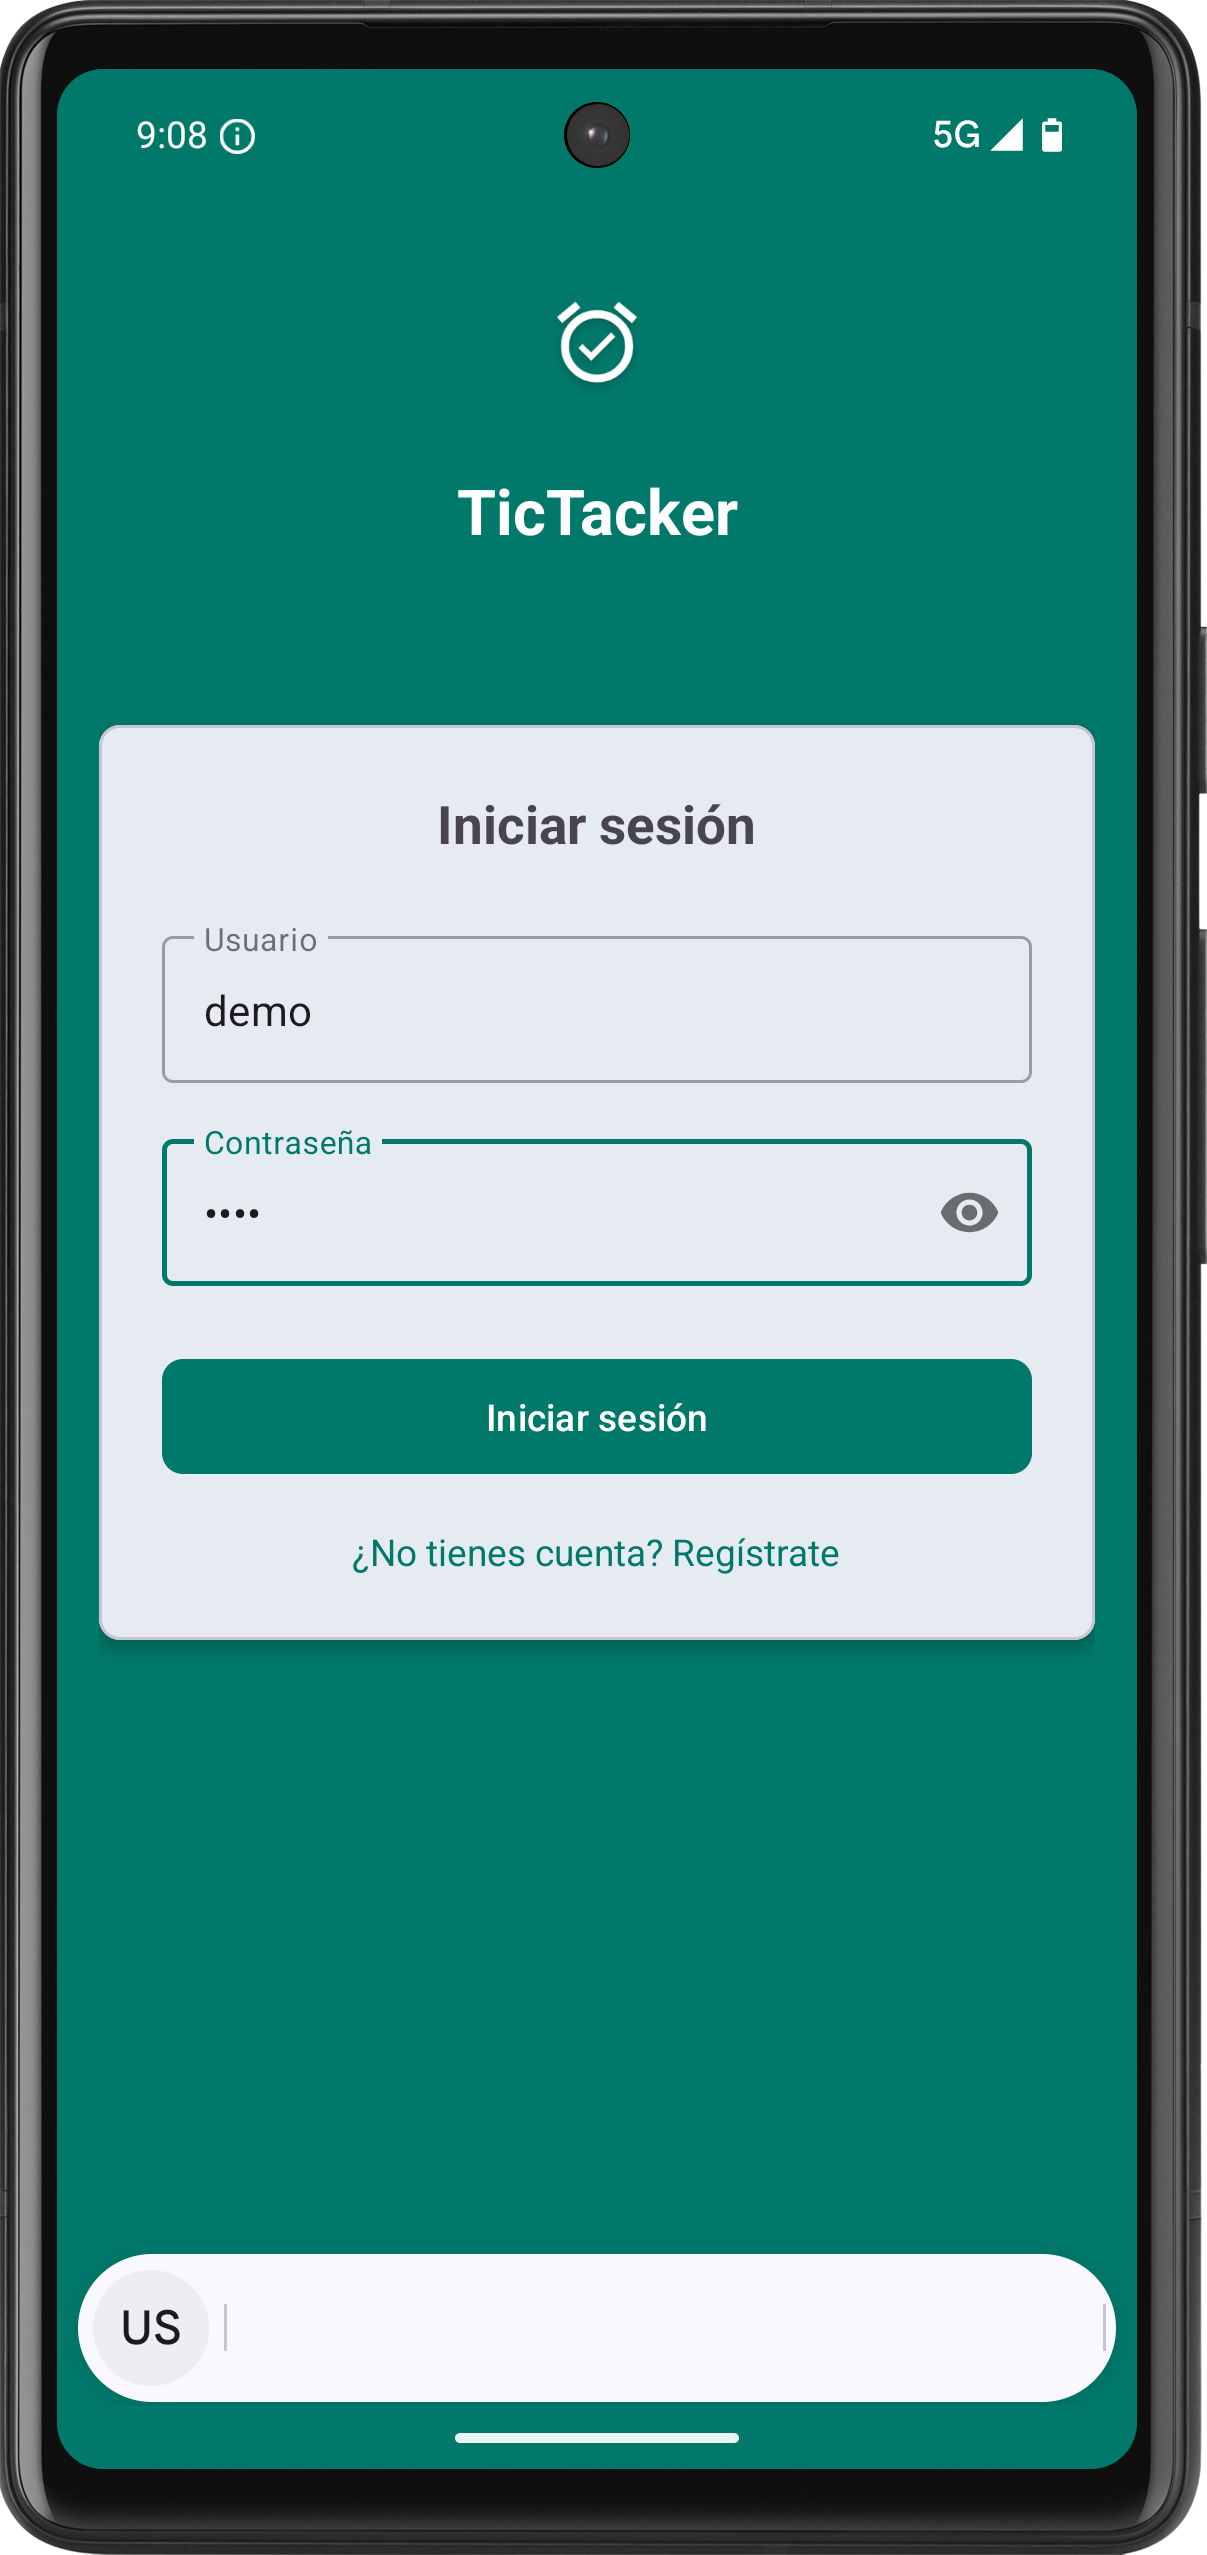
\includegraphics[width=\textwidth]{root/login.png}
         \caption{Inicio de sesión}
         \label{fig:login}
     \end{subfigure}
     \hfill
     \begin{subfigure}[b]{0.3\textwidth}
         \centering
         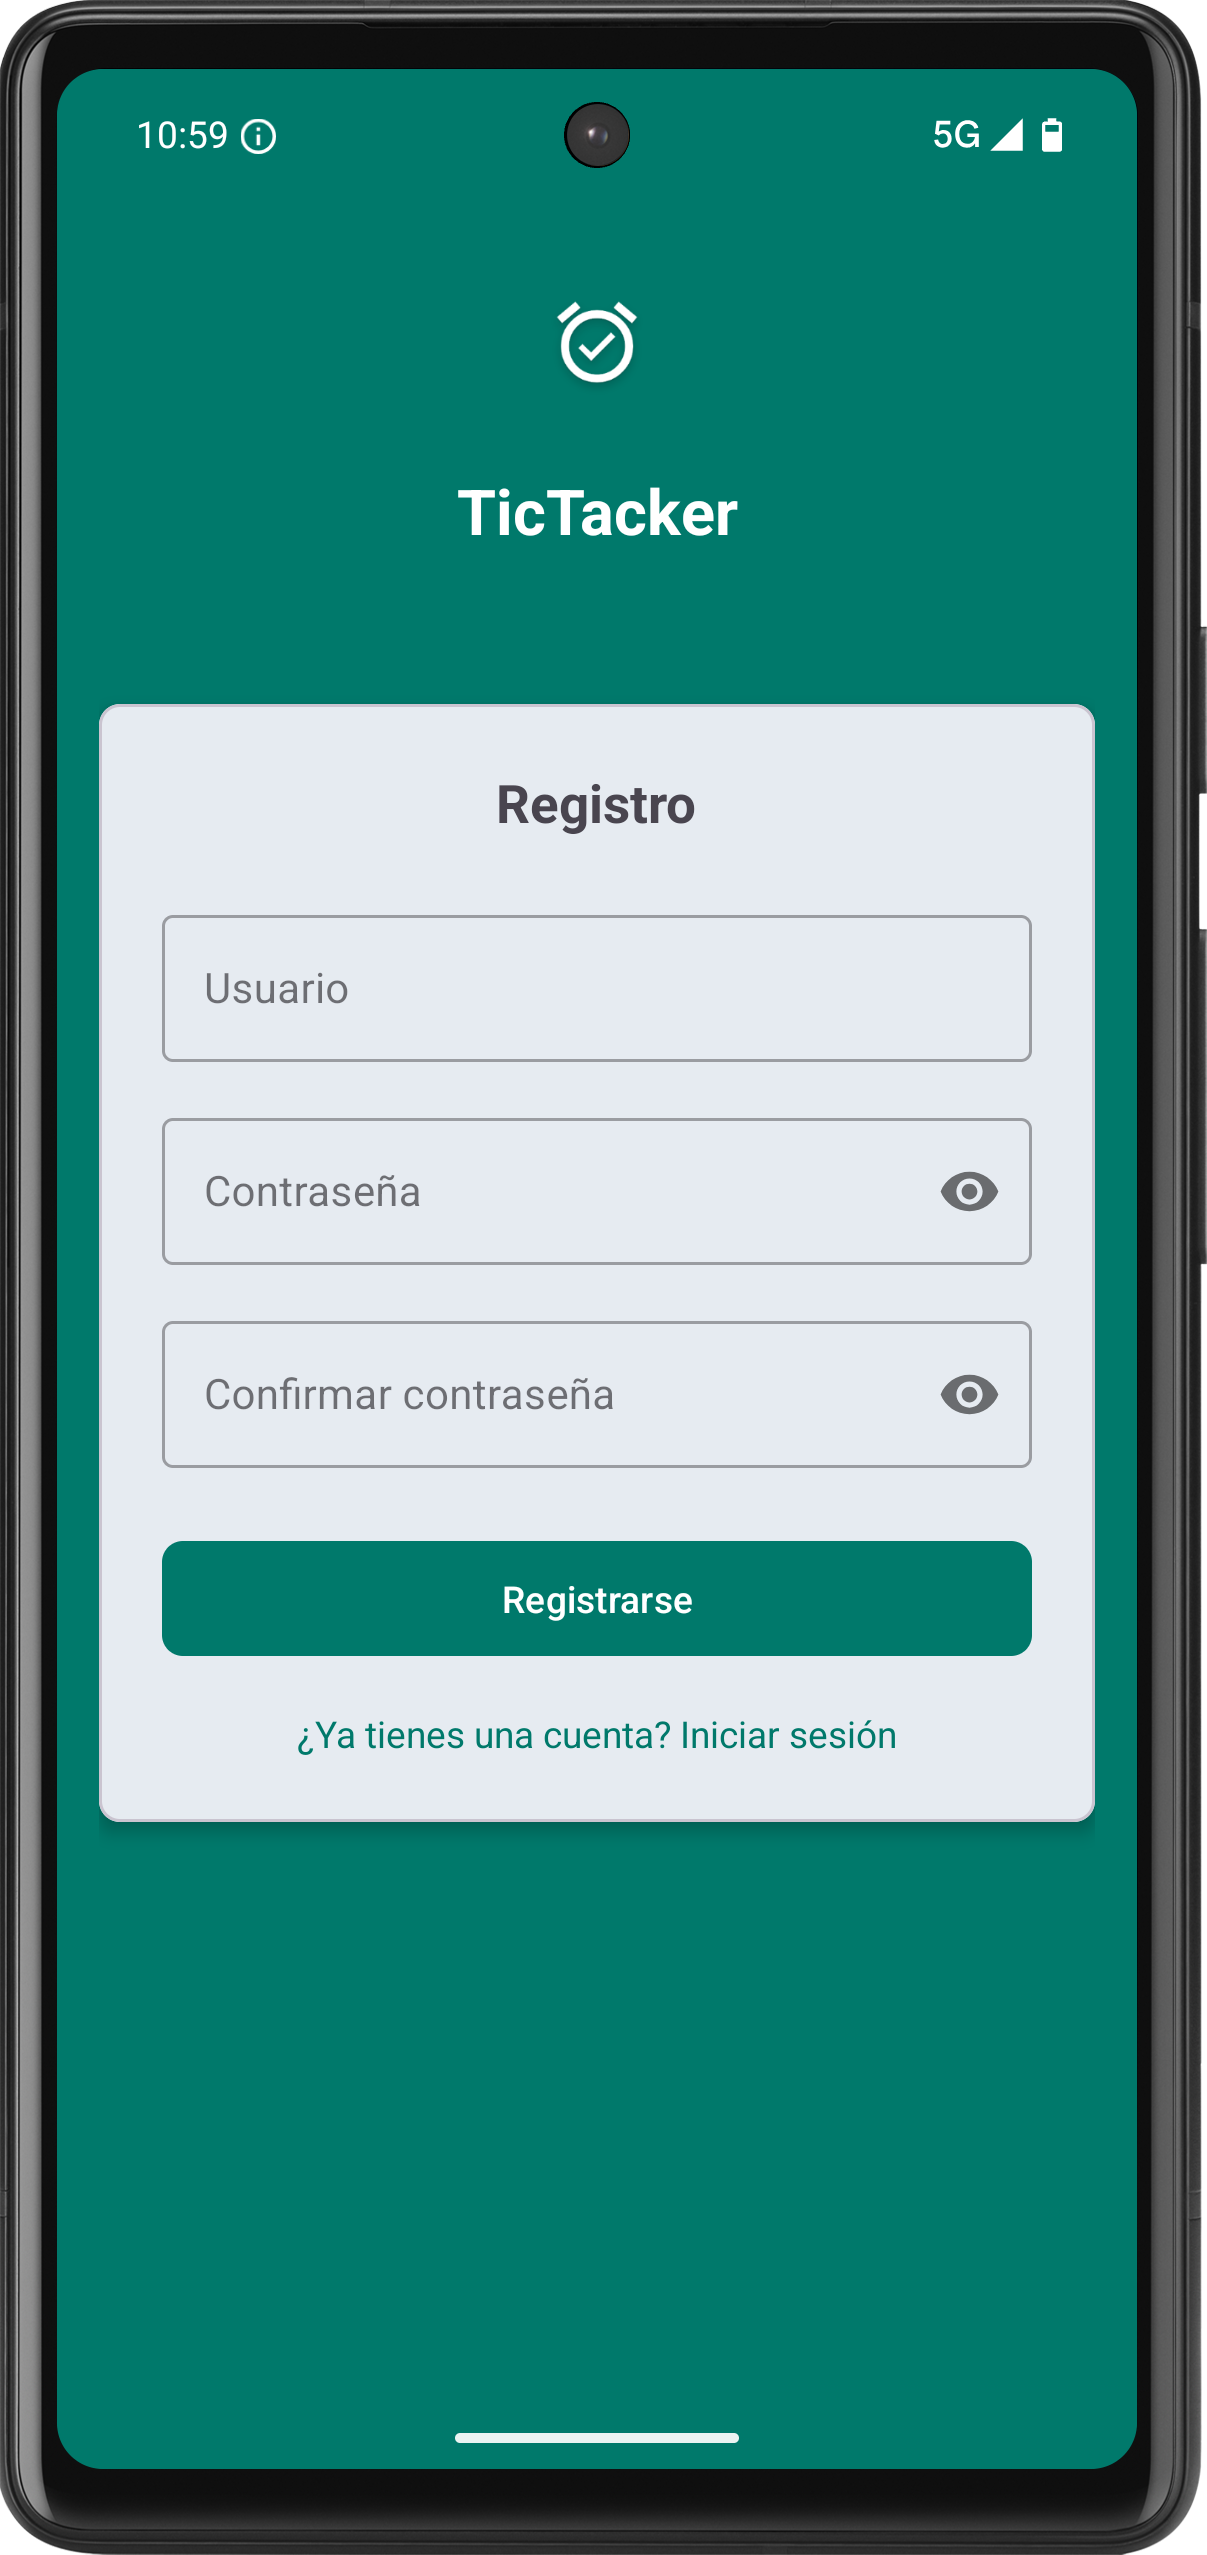
\includegraphics[width=\textwidth]{root/signup.png}
         \caption{Registro de usuario}
         \label{fig:signup}
     \end{subfigure}
     \hfill
     \begin{subfigure}[b]{0.3\textwidth}
         \centering
         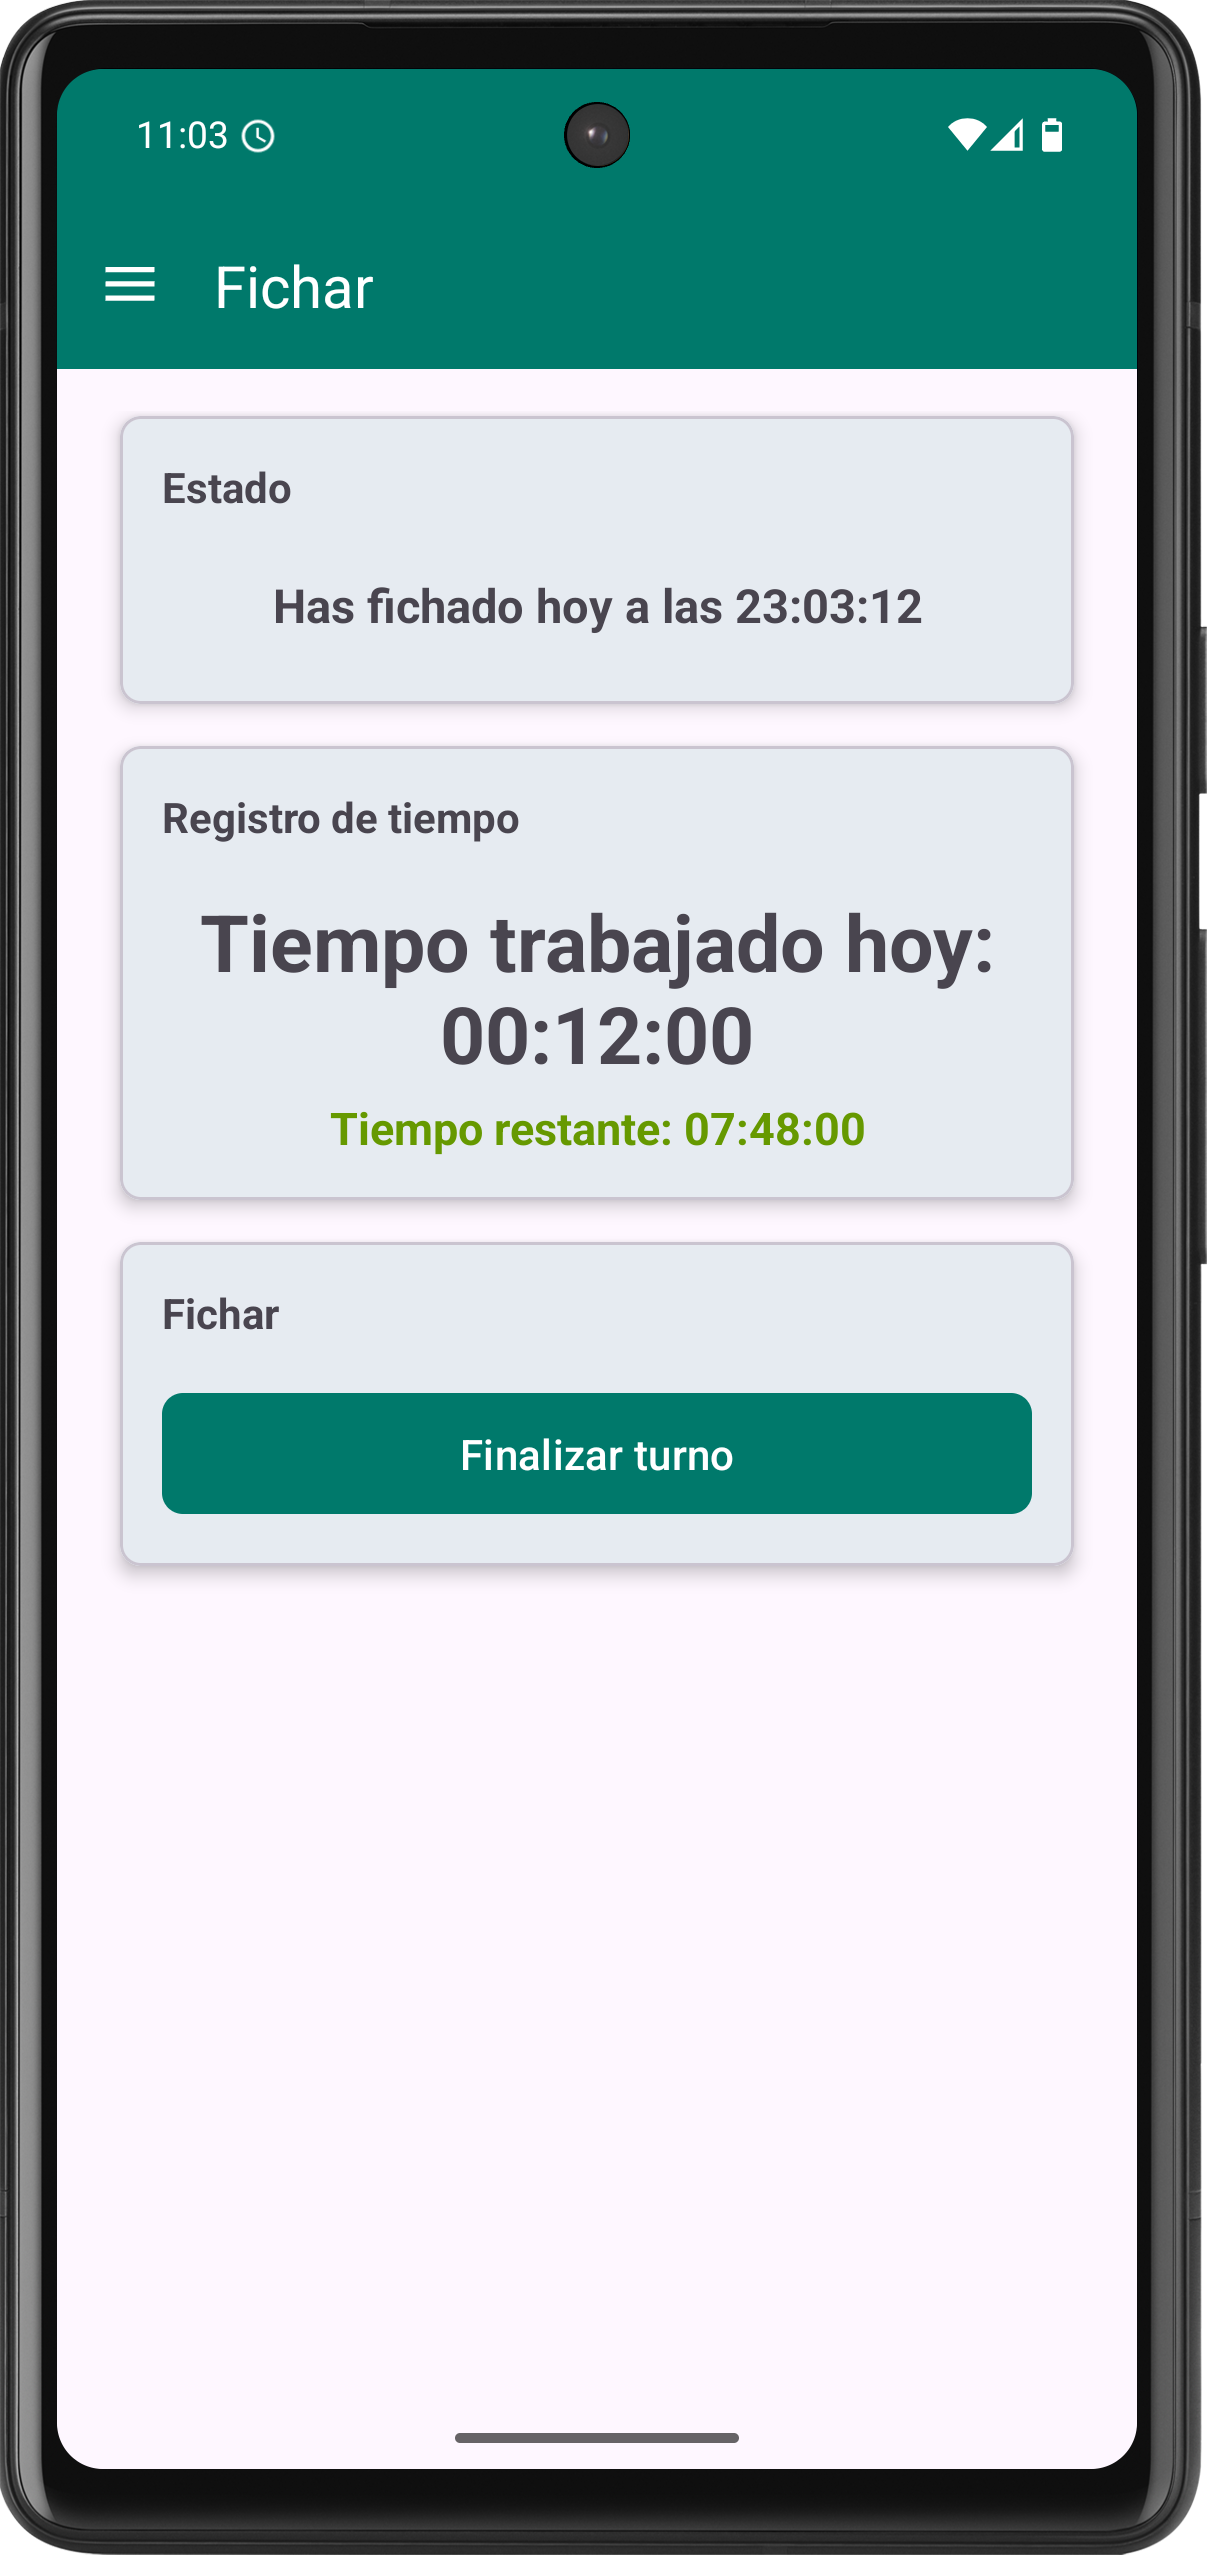
\includegraphics[width=\textwidth]{root/fichado.png}
         \caption{Pantalla de inicio}
         \label{fig:fichado}
     \end{subfigure}
        \caption{Pantalla de bienvenida e inicio de sesión}
        \label{fig:bienvenida}
\end{figure}

\subsection{Ajustes de la aplicación}

Pulsando sobre la sección de “Ajustes” en el menú de la aplicación, se accederá a la configuración. Es importante presionar sobre el botón de “Guardar” para que se refresque la vista de la aplicación y se puedan ver los cambios realizados de forma correcta si se modifica alguno de los capos.

Para obtener la mejor experiencia posible, se permite elegir, tal y como se muestra en la Figura \ref{fig:settings-1}, entre Español e Inglés como idiomas, siendo suficiente con elegir en el desplegable el preferido para configurarlo como el idioma por defecto para toda la aplicación. A continuación, el usuario deberá completar los datos de su jornada laboral, especificando los días laborables y las horas que se trabaja a la semana usando los controles. Esta información permite a la aplicación calcular las horas que se trabajará cada día, así como enviar notificaciones en caso de superar la previsión diaria y mostrar un cuadro de diálogo si se trata de salir antes de lo previsto.

De forma opcional, es posible incluir una imagen como logotipo, que se mostrará en el menú de la aplicación tal y como ilustra la Figura \ref{fig:settings-3}. Para ello, basta con pulsar sobre el botón de “Cambiar” y elegir el nuevo logotipo en el explorador, como muestra la Figura \ref{fig:settings-2}. Debe ser un fichero de imagen, y se recomienda que sea un PNG con fondo transparente y un color claro para mejor visibilidad. En caso de querer restaurar el logotipo por defecto, puede usarse el botón de “Quitar”.

De forma adicional, esta pantalla también permite cerrar sesión para cambiar de usuario, lo que nos llevaría directamente a la pantalla de inicio de sesión, así como eliminar los datos de fichaje almacenados, lo que no se recomienda salvo que se hayan exportado previamente.

\begin{figure}[H]
     \centering
     \begin{subfigure}[b]{0.3\textwidth}
         \centering
         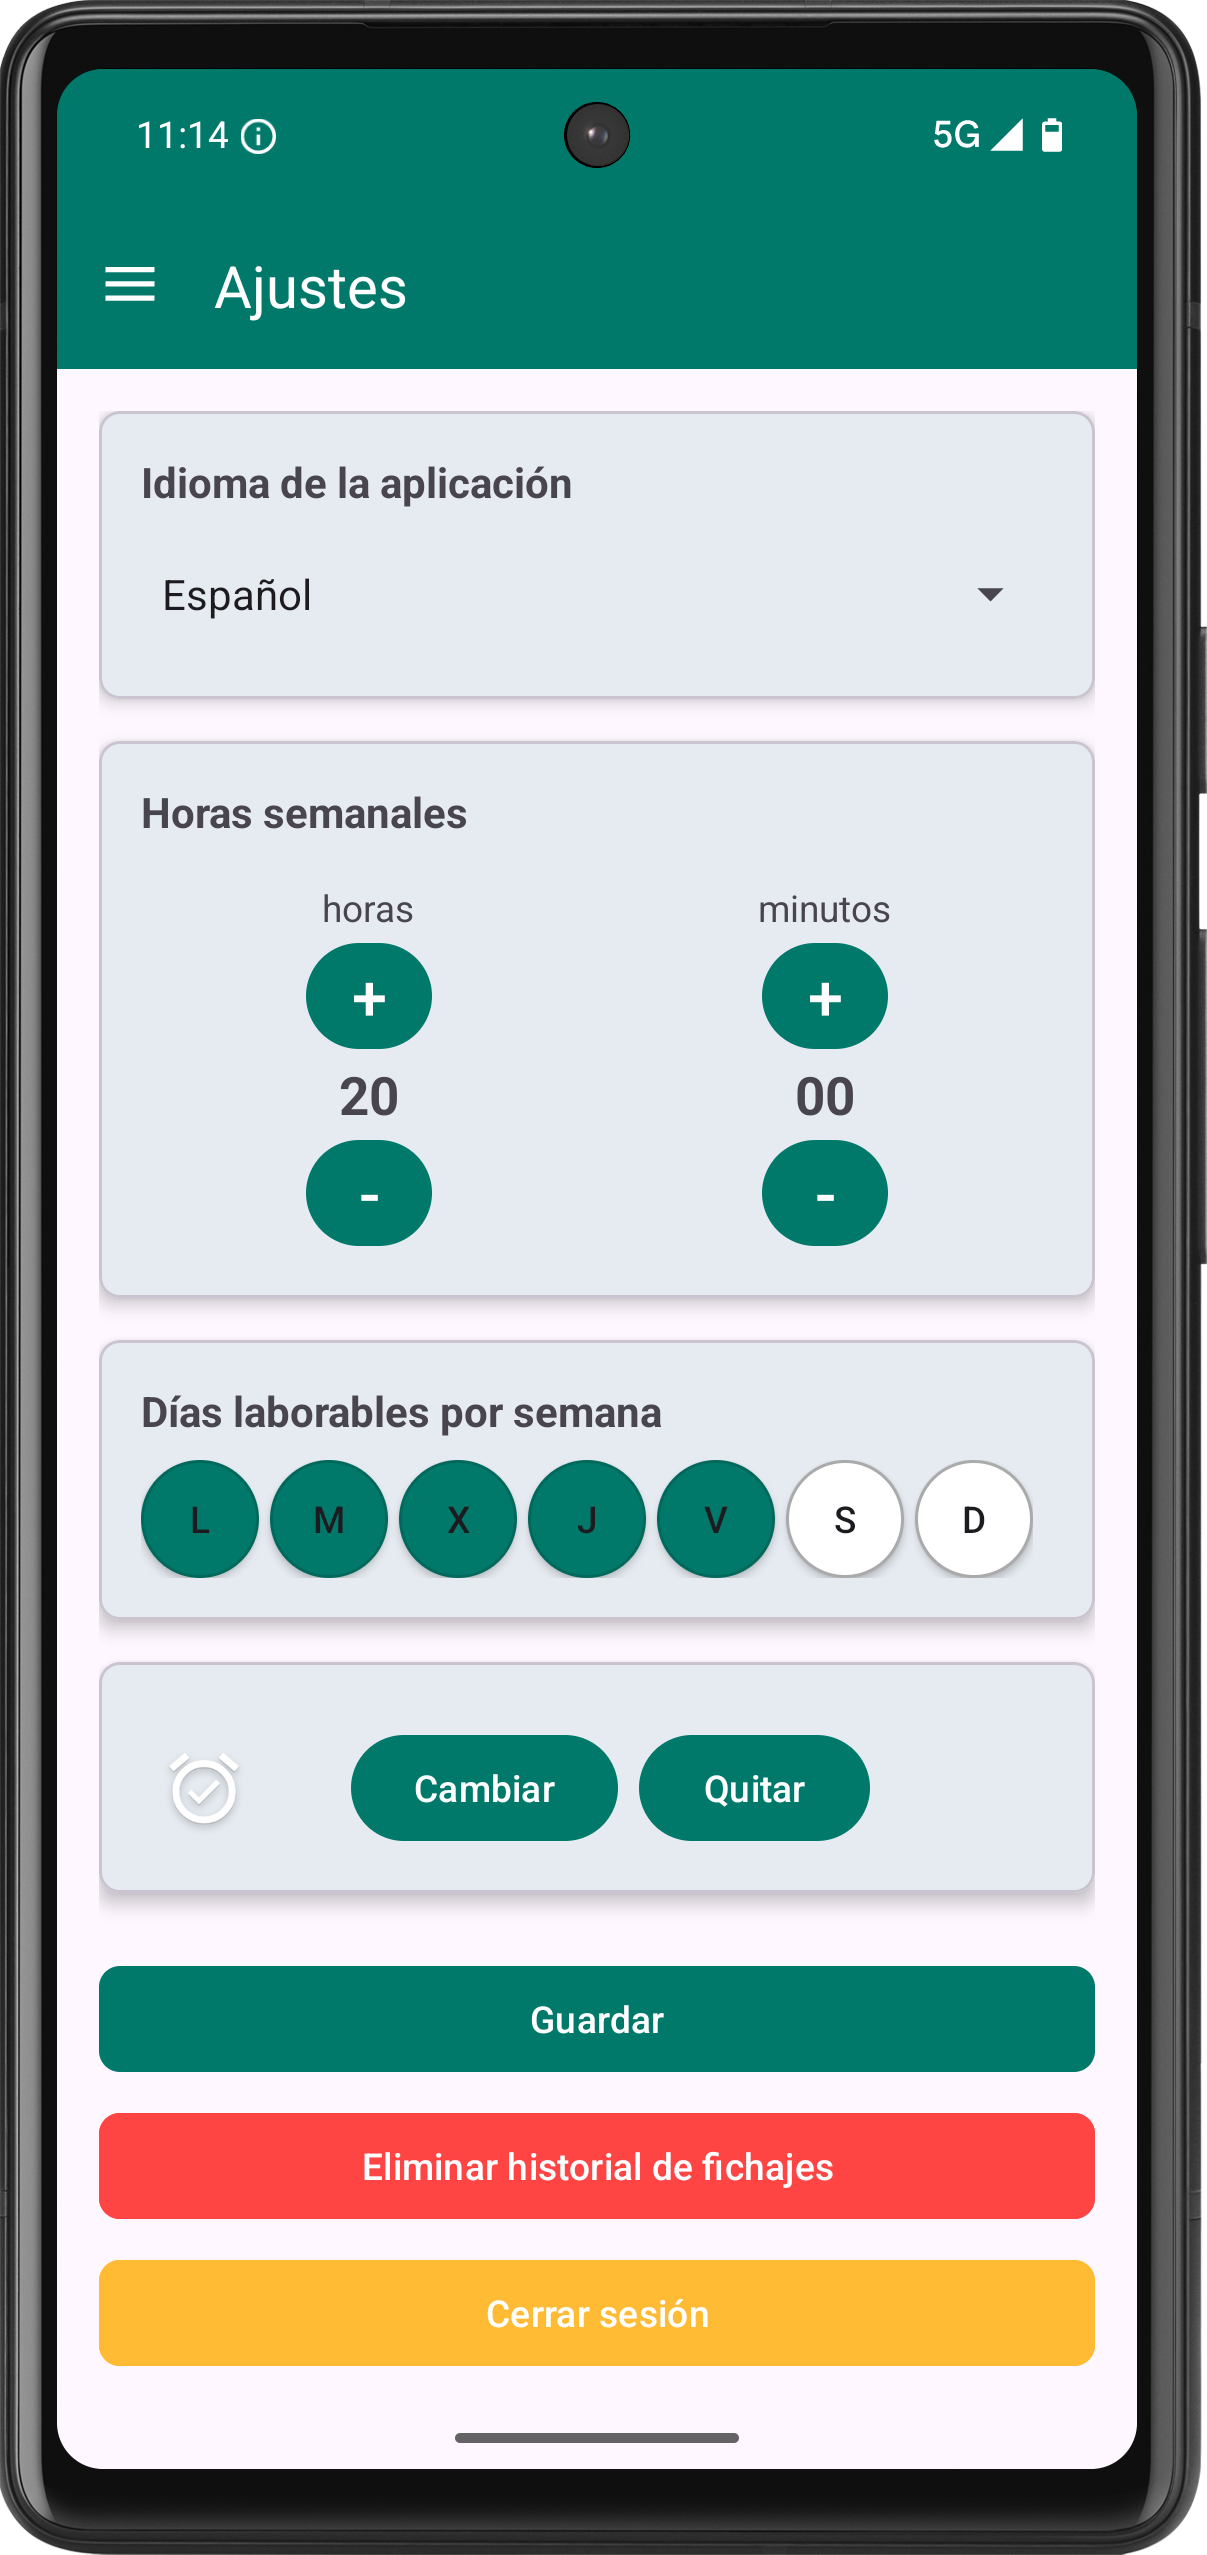
\includegraphics[width=\textwidth]{root/settings-1.png}
         \caption{Ajustes de la aplicación}
         \label{fig:settings-1}
     \end{subfigure}
     \hfill
     \begin{subfigure}[b]{0.3\textwidth}
         \centering
         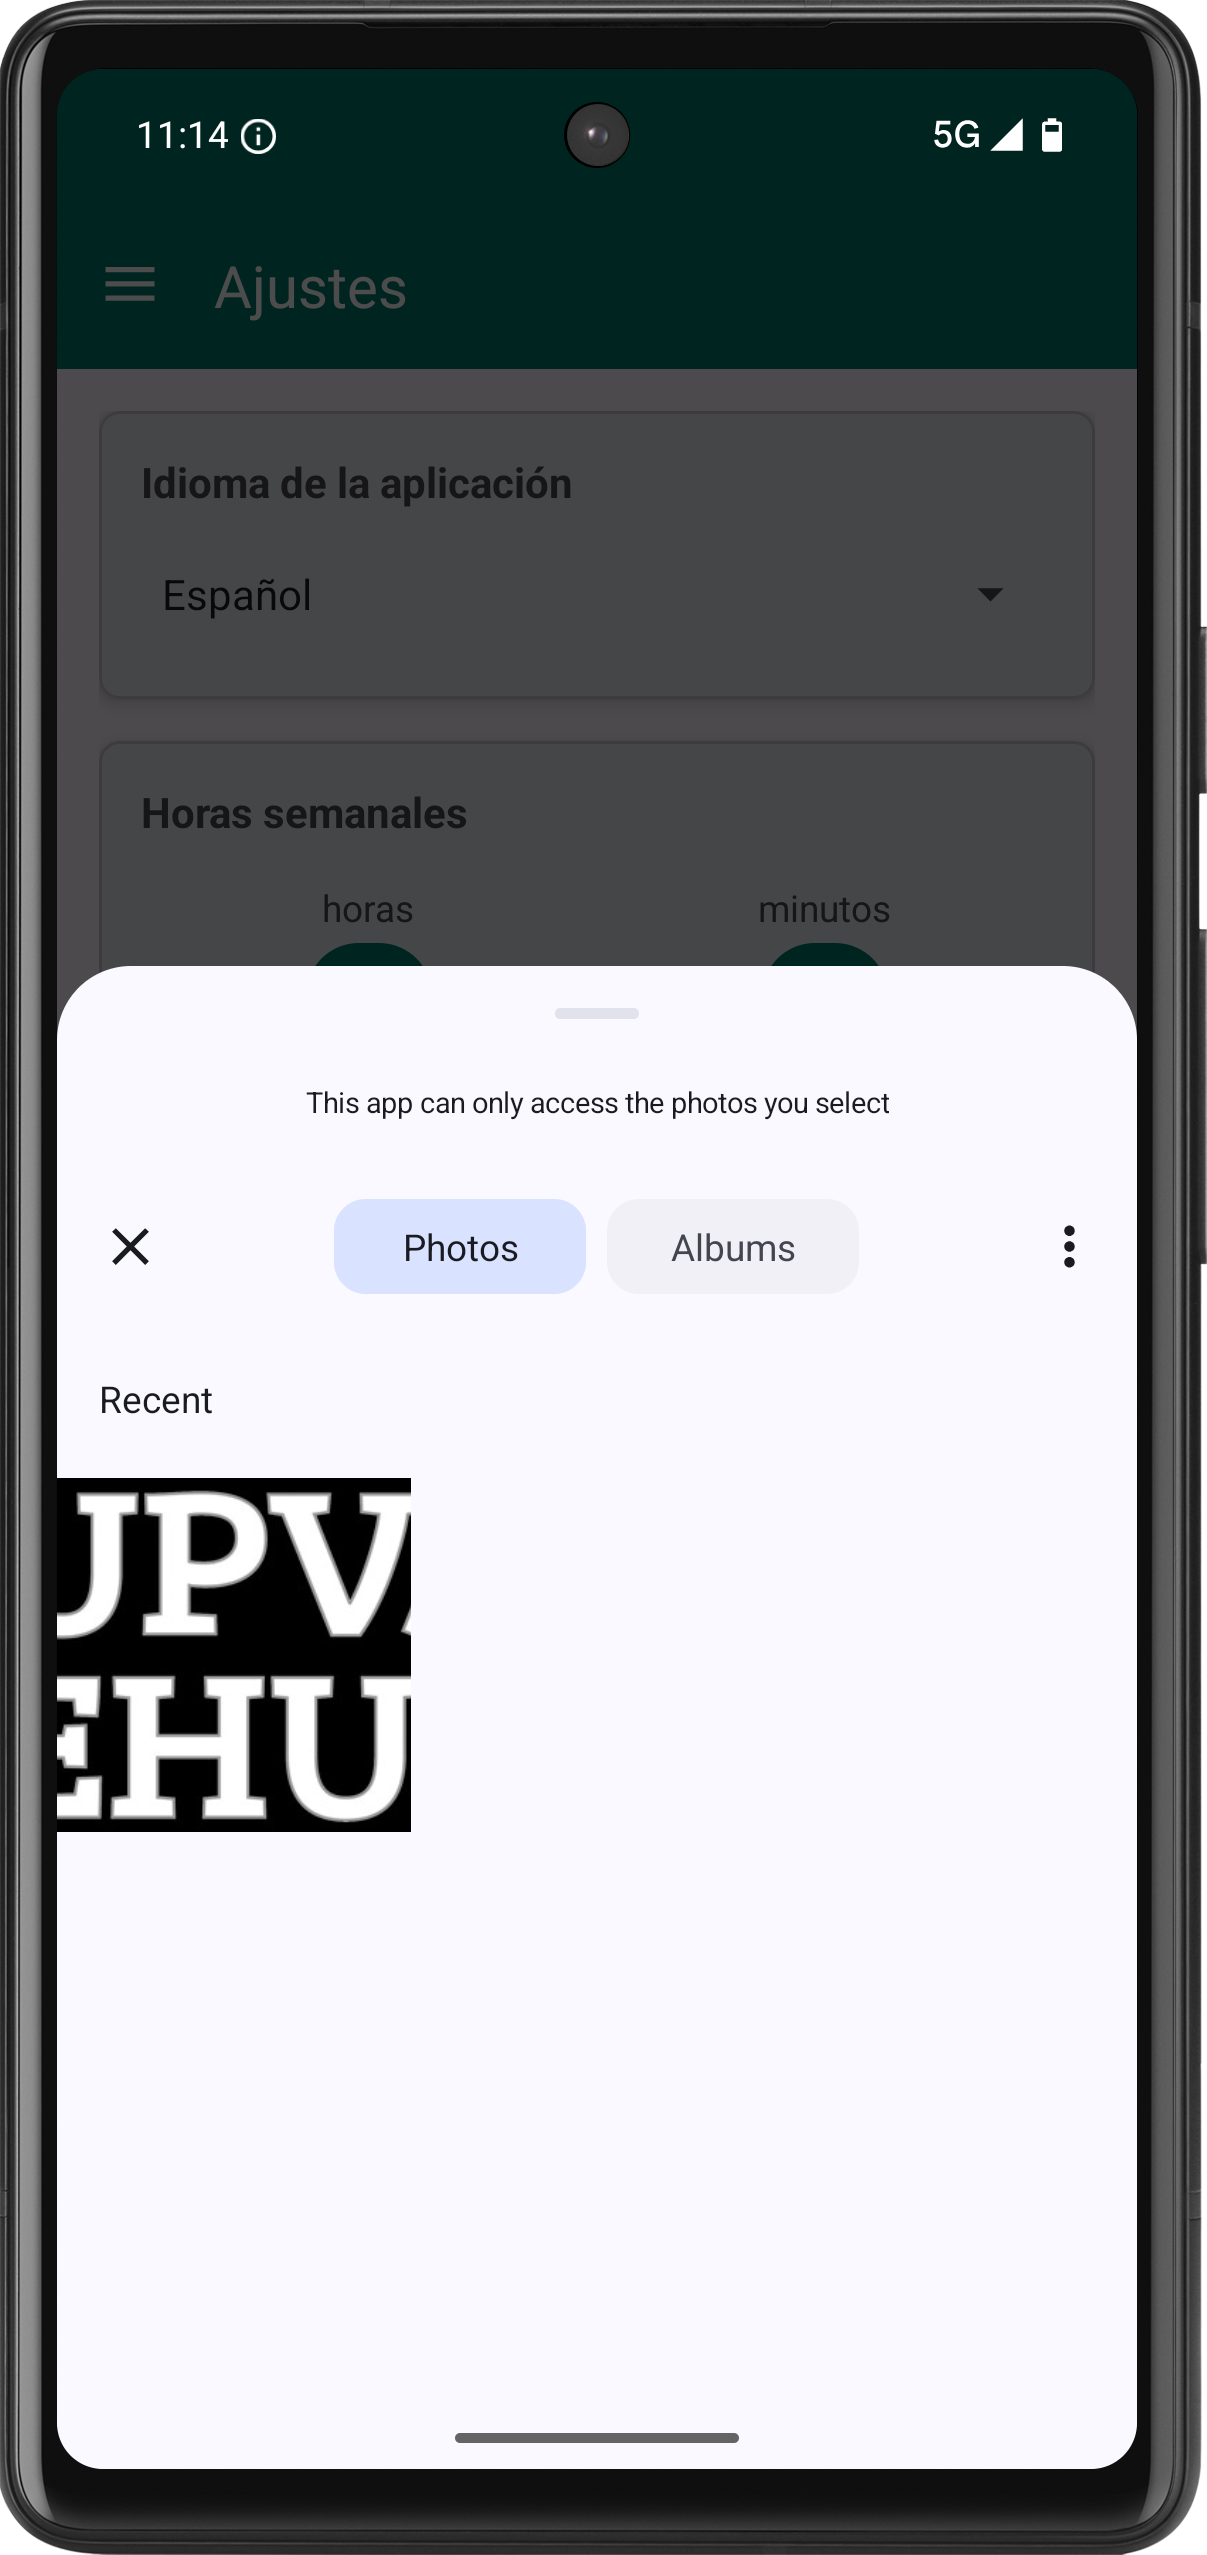
\includegraphics[width=\textwidth]{root/settings-2.png}
         \caption{Selección de nuevo logotipo}
         \label{fig:settings-2}
     \end{subfigure}
     \hfill
     \begin{subfigure}[b]{0.3\textwidth}
         \centering
         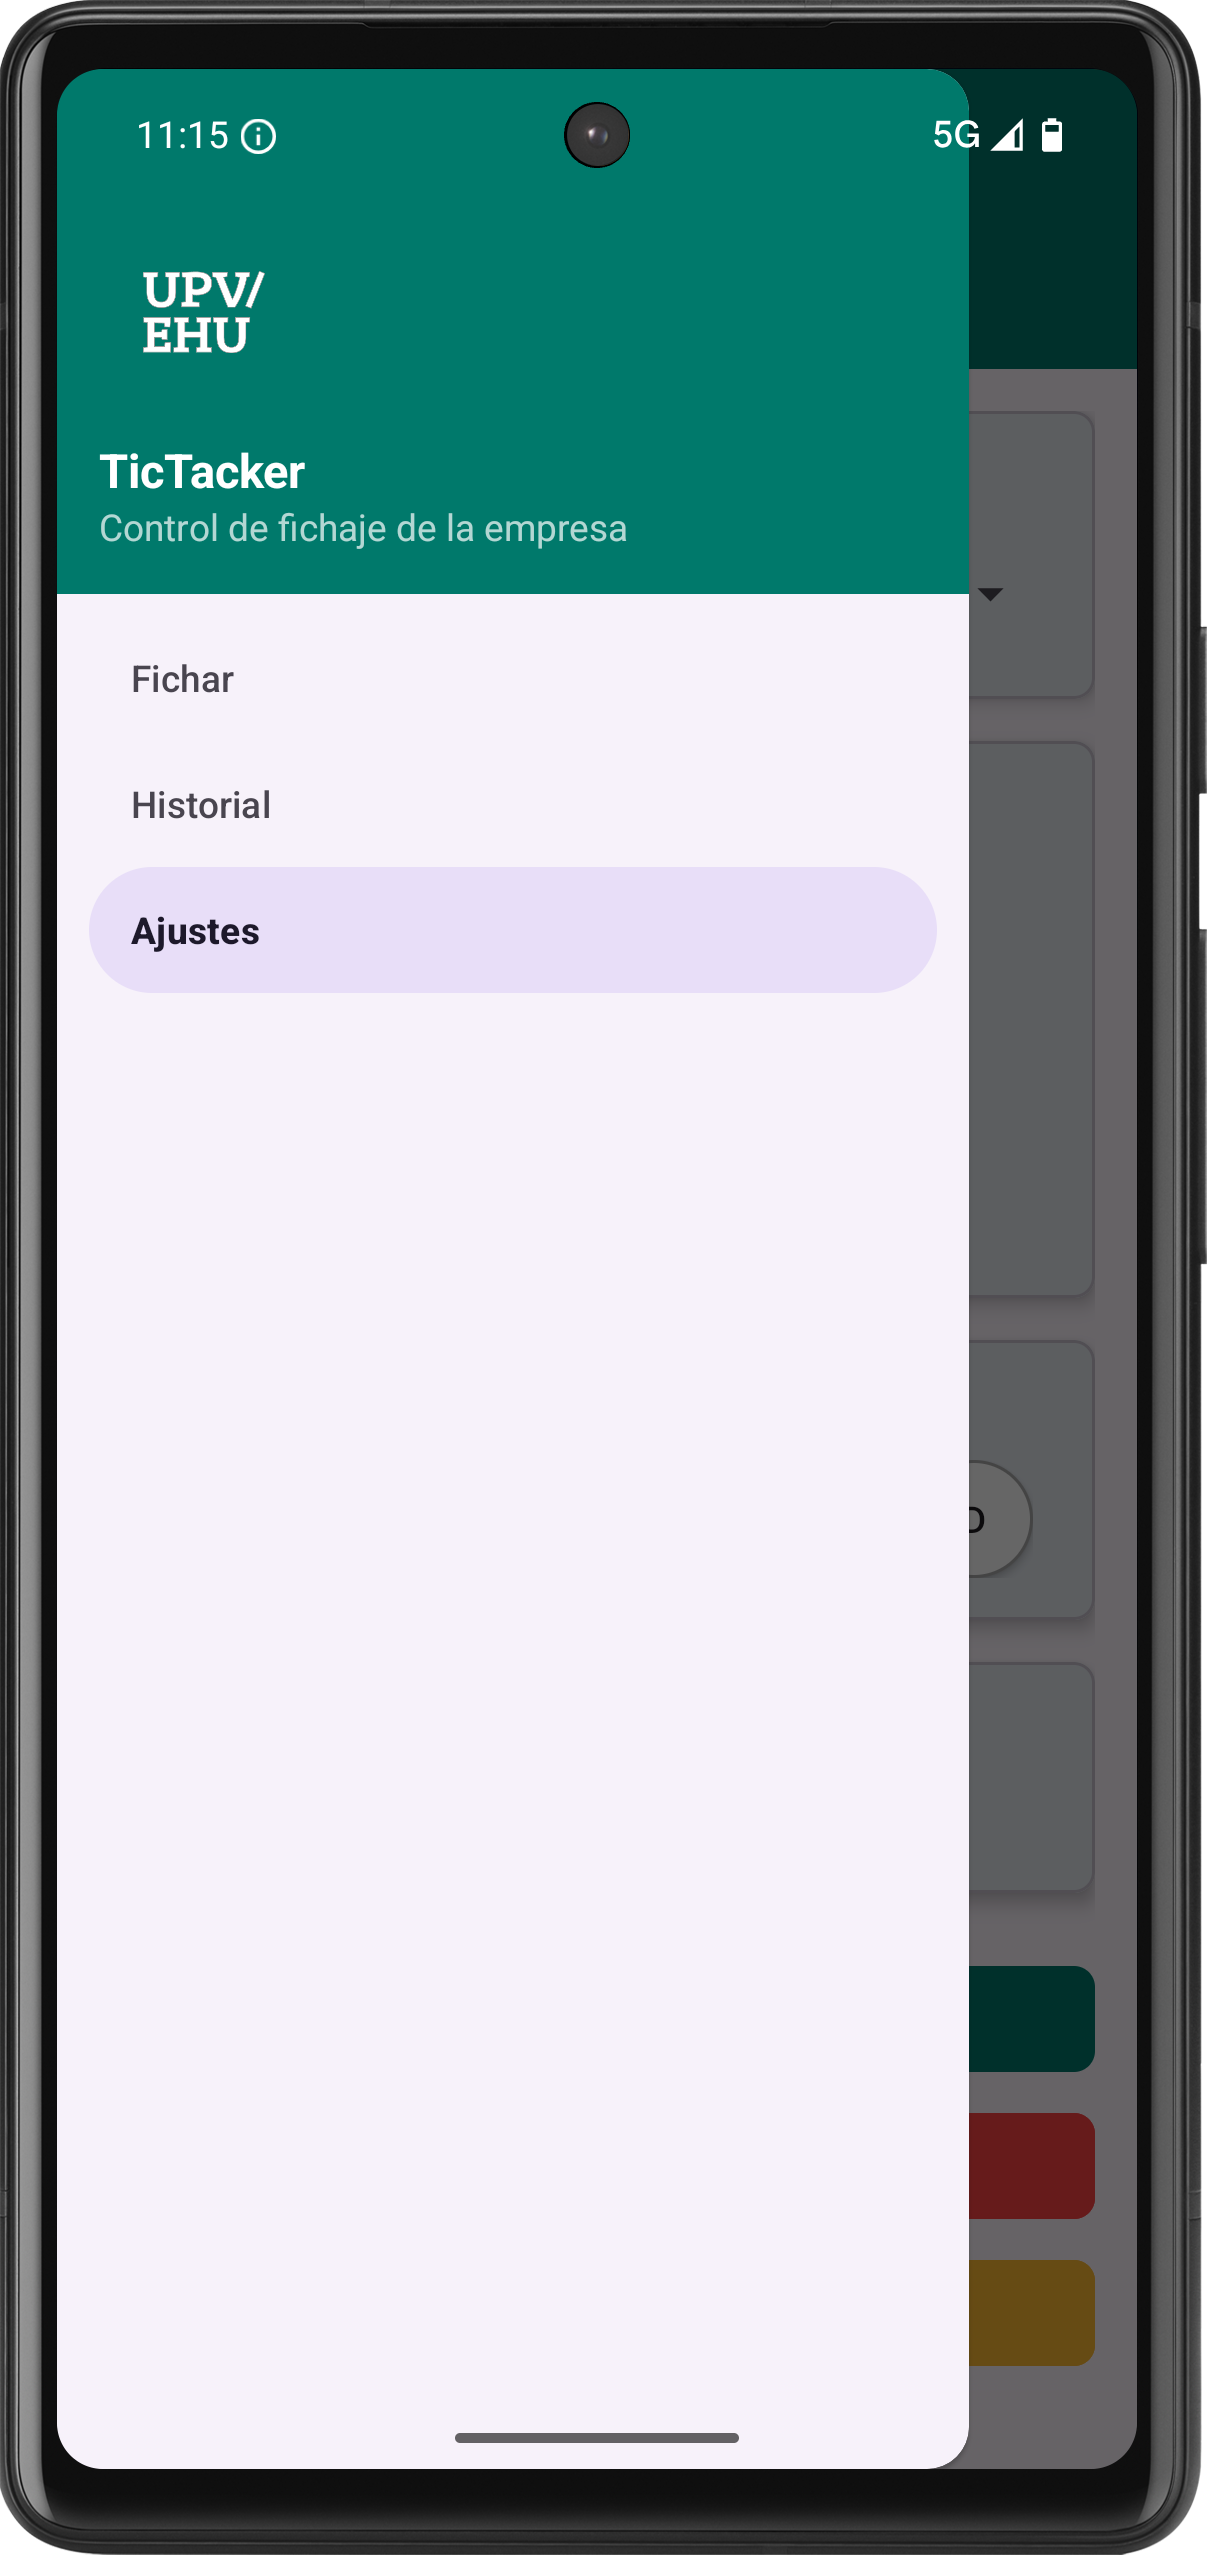
\includegraphics[width=\textwidth]{root/settings-3.png}
         \caption{Navegación con logotipo}
         \label{fig:settings-3}
     \end{subfigure}
        \caption{Ajustes de la aplicación}
        \label{fig:bienvenida}
\end{figure}

\subsection{Fichajes e historial}

Accediendo a la pantalla para fichar, es posible consultar de un vistazo los datos de un fichaje activo, tal y como muestra la Figura \ref{fig:fichando}. Es posible marcar una entrada y una salida por medio del botón asociado de forma sencilla, y consultar la hora, minuto y segundo exacto en el que se fichó, así como la duración actual, el tiempo restante para alcanzar la jornada o, en su defecto, las horas extraordinarias realizadas. Al llegar a las horas estimadas, se recibe una notificación si la aplicación está activa.

Una vez guardado el fichaje, desde el menú es posible acceder al historial que muestra la figura \ref{fig:historial}. En él, puede verse un registro de todos los fichajes almacenados en la aplicación, mostrándose primero el más reciente. Si se pulsa sobre uno de ellos, como se muestra en la Figura \ref{fig:detalles}, es posible ver el detalle completo, consultando la fecha y hora exactas de salidas y entradas, así como las coordenadas geográficas desde las que se produjo el fichaje en caso de haber otorgado permisos para acceder a la ubicación (en su defecto, se mostrará que no está disponible).

En la parte inferior de la ventana de detalles, existen opciones para editar un fichaje guardado, que permite modificar la hora de entrada o salida en caso de haberse identificado algún error, así como la opción de ver en un mapa la ubicación registrada. Al pulsar sobre esta opción, se abre la aplicación de mapas asociada del dispositivo (Google Maps en gran parte de las ocasiones).

\begin{figure}[H]
     \centering
     \begin{subfigure}[b]{0.3\textwidth}
         \centering
         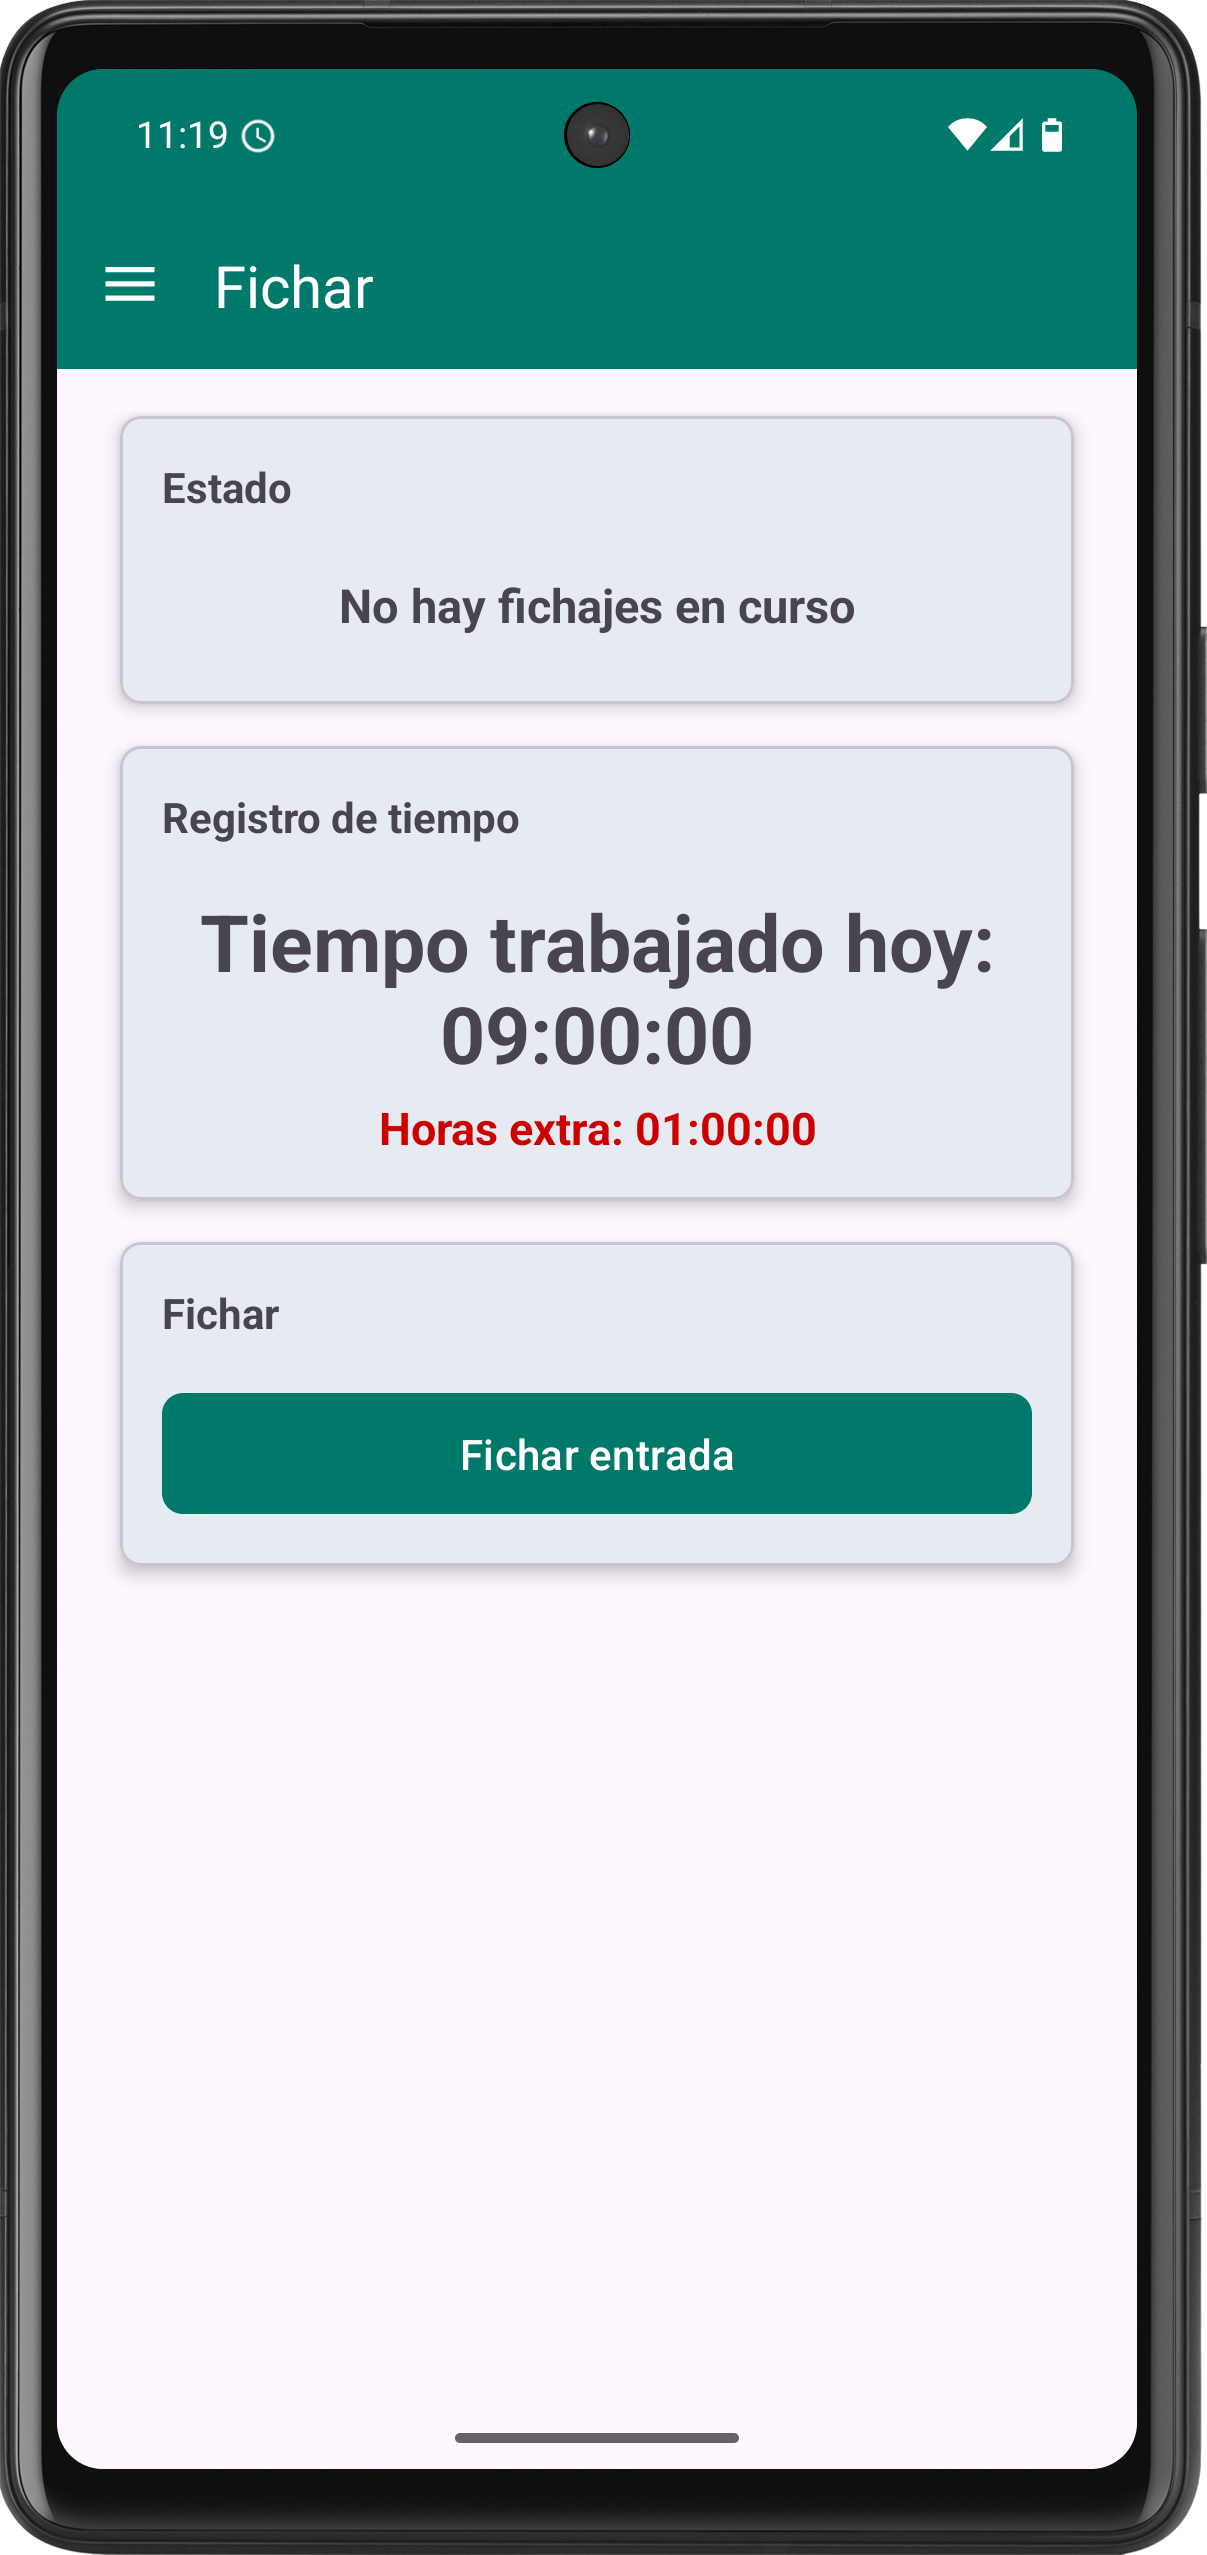
\includegraphics[width=\textwidth]{root/fichando.png}
         \caption{Pantalla de fichaje}
         \label{fig:fichando}
     \end{subfigure}
     \hfill
     \begin{subfigure}[b]{0.3\textwidth}
         \centering
         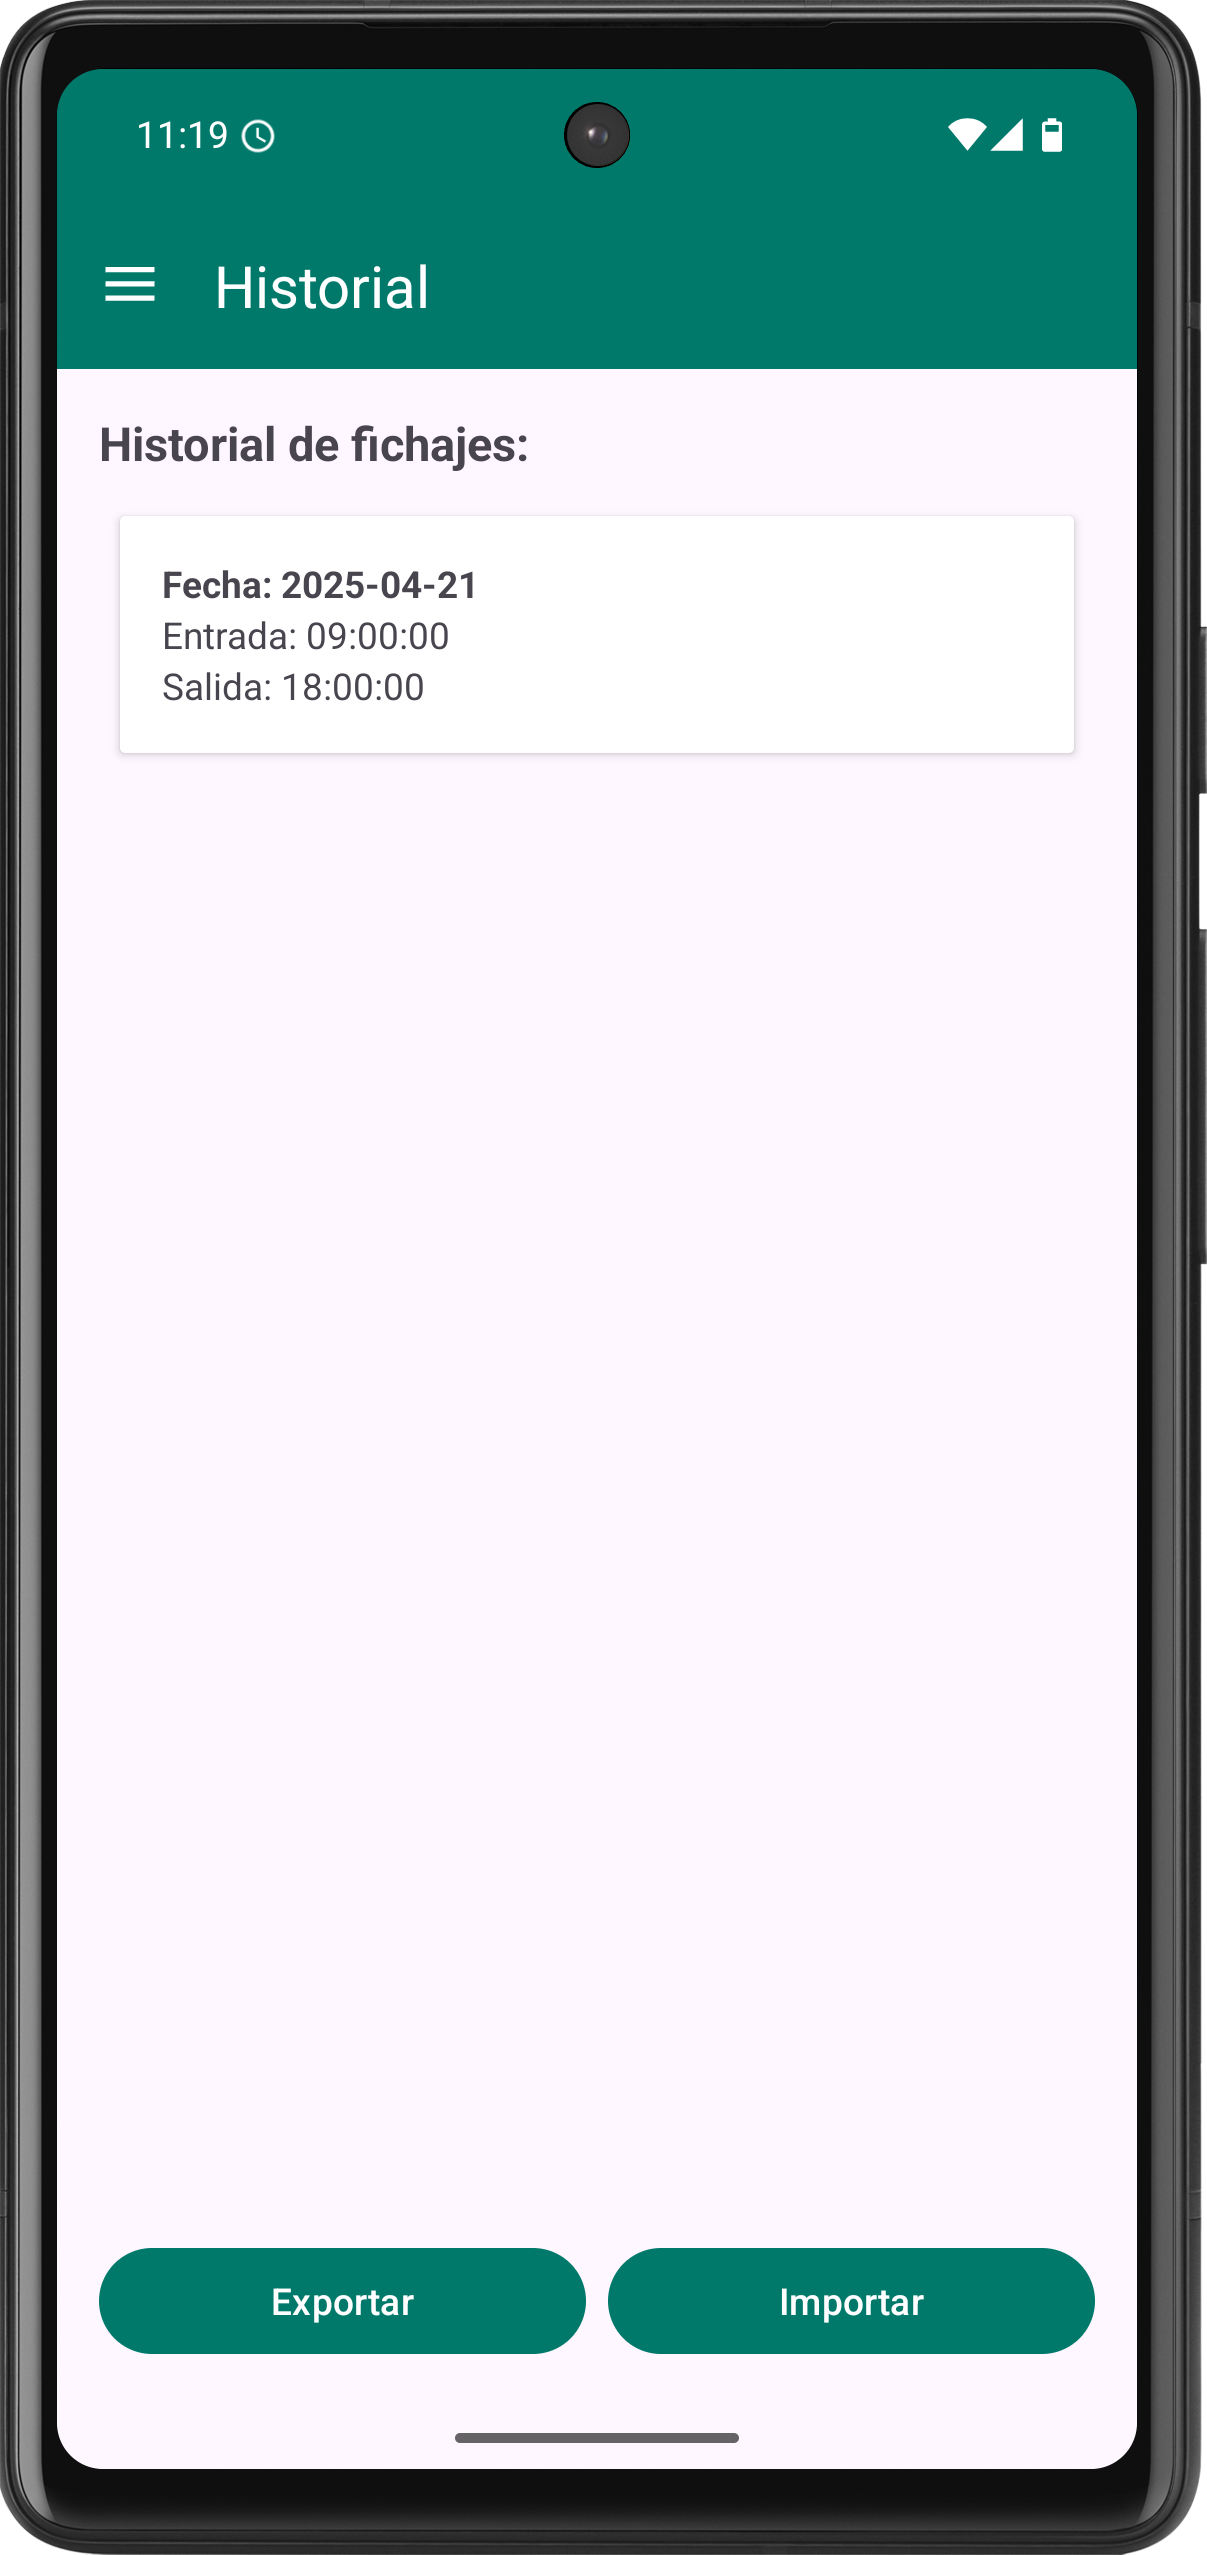
\includegraphics[width=\textwidth]{root/historial.png}
         \caption{Historial de fichajes}
         \label{fig:historial}
     \end{subfigure}
     \hfill
     \begin{subfigure}[b]{0.3\textwidth}
         \centering
         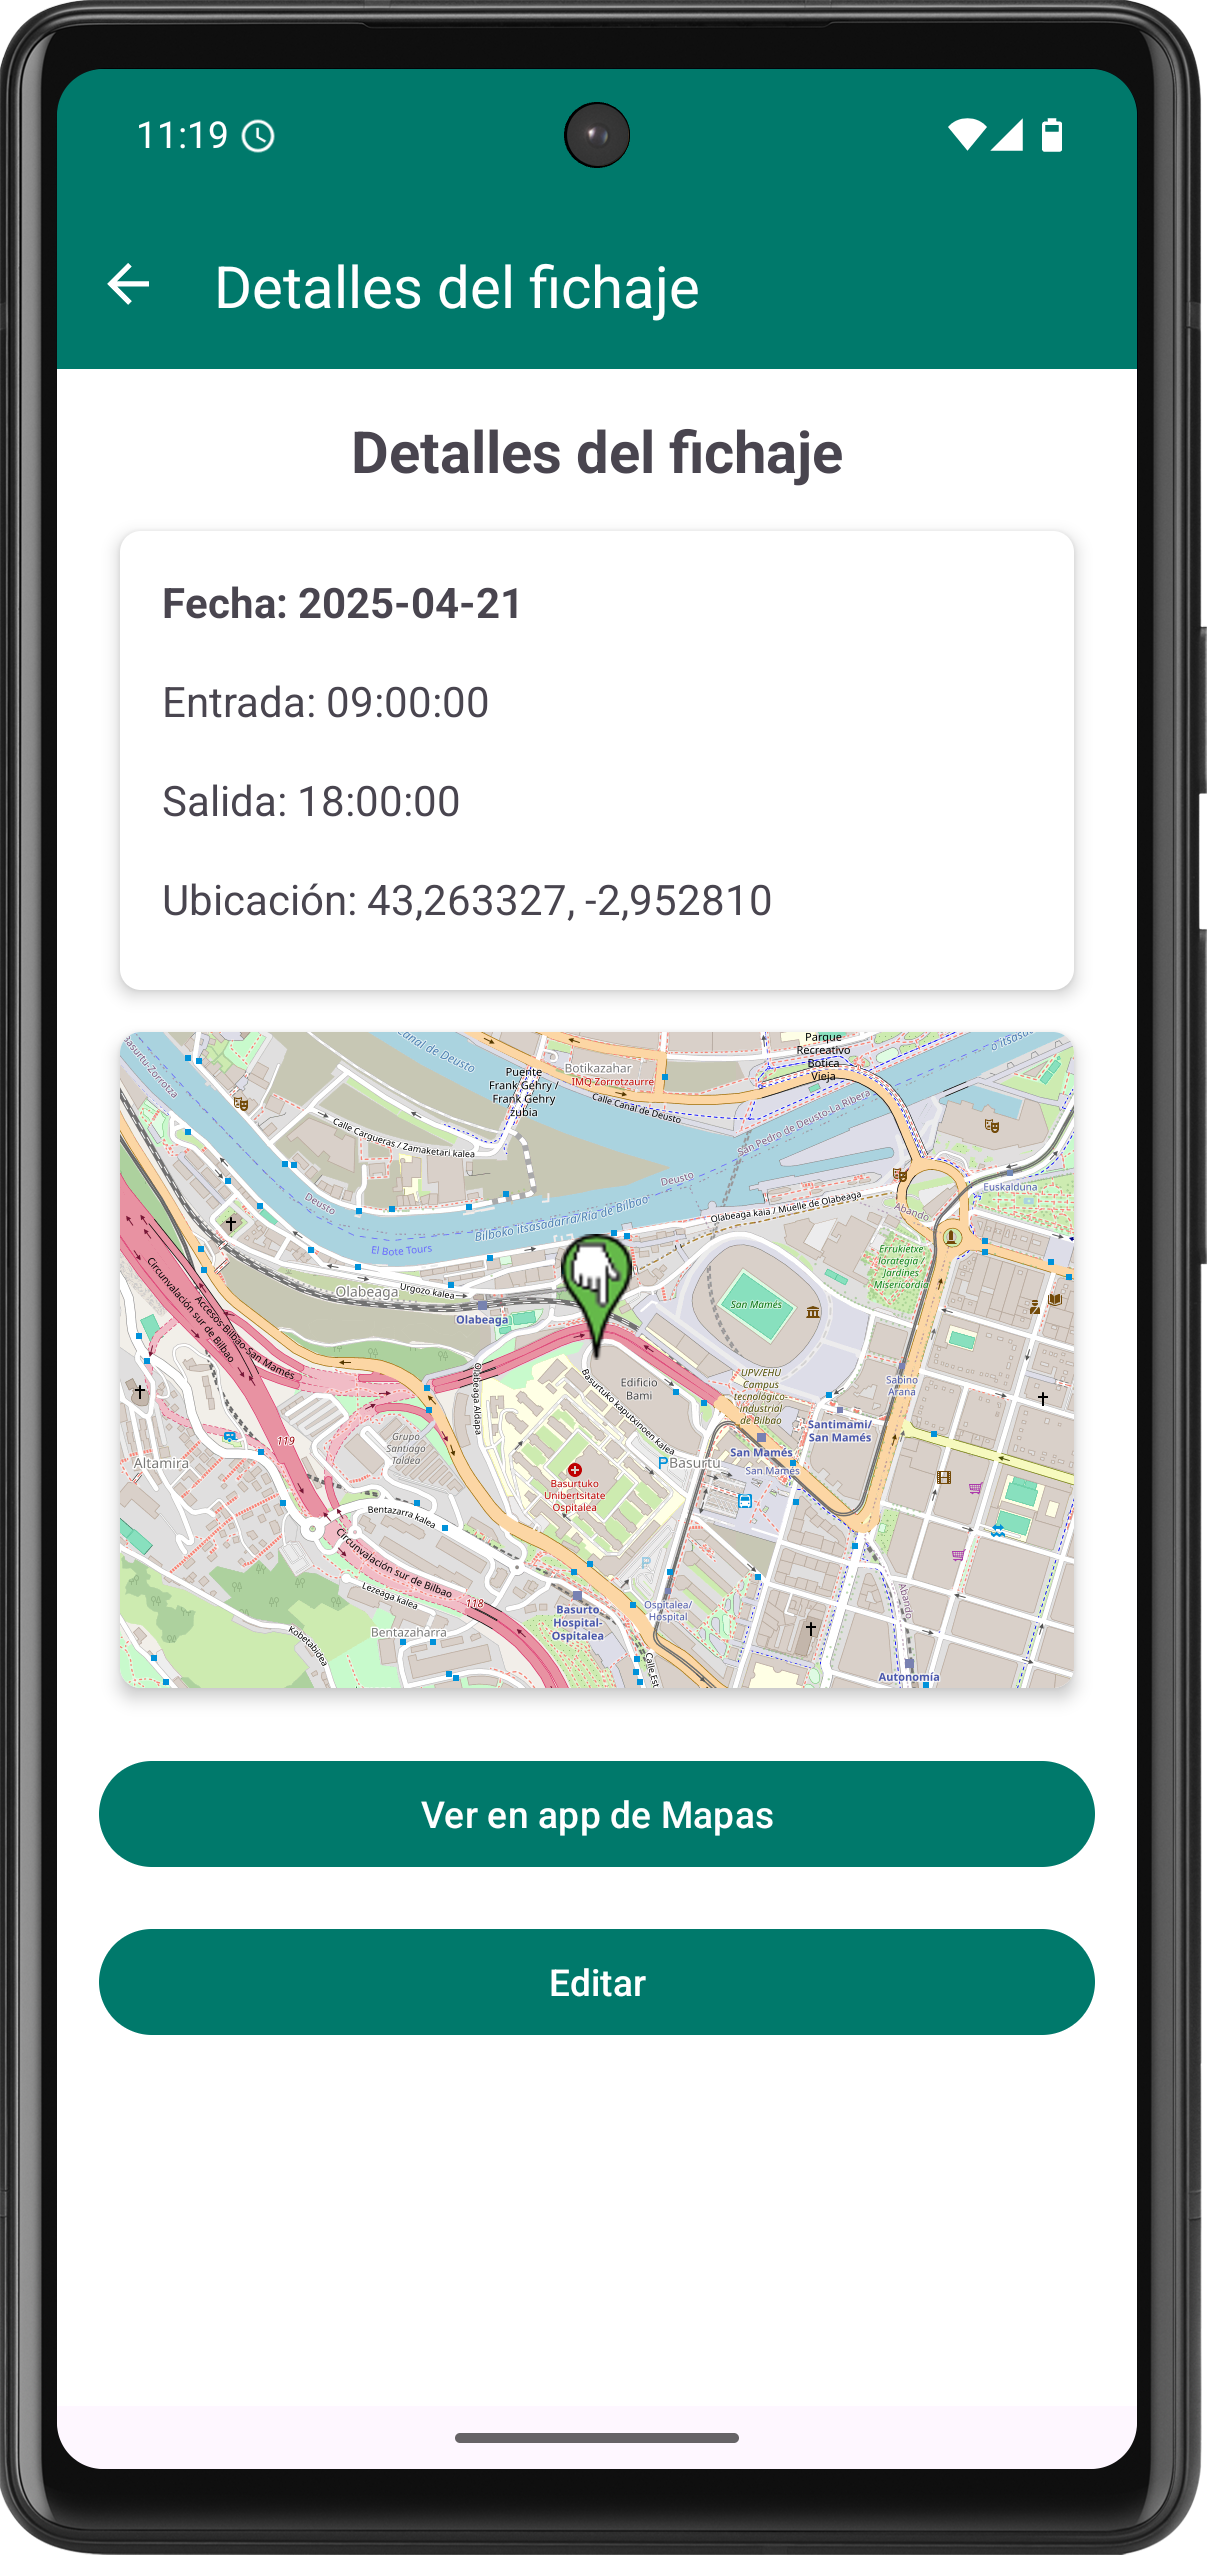
\includegraphics[width=\textwidth]{root/detalles.png}
         \caption{Detalles de un fichaje}
         \label{fig:detalles}
     \end{subfigure}
        \caption{Uso general de la aplicación}
        \label{fig:uso}
\end{figure}

De forma adicional, la parte inferior de la aplicación permite importar o exportar una hoja de fichajes. Al presionar sobre exportar, se genera un fichero CSV con los fichados registrados, para el que deberá elegirse una ubicación dentro del dispositivo en la que guardarlo, mientras que si se selecciona importar, se puede elegir un fichero generado previamente por la aplicación o de forma manual con el mismo formato. Al hacerlo, se almacenarán los detalles en la base de datos y se podrá ver en el historial junto al resto de datos.